\chapter{Interface gráfica}
\label{interface}

A interface gráfica é responsável pela interação com o usuário.
Nela, o usuário escreve o programa, visualiza e interage com os objetos.
A Figura \ref{img:comp} ilustra os componentes da interface gráfica.

\begin{figure}[!ht]
    \centering
    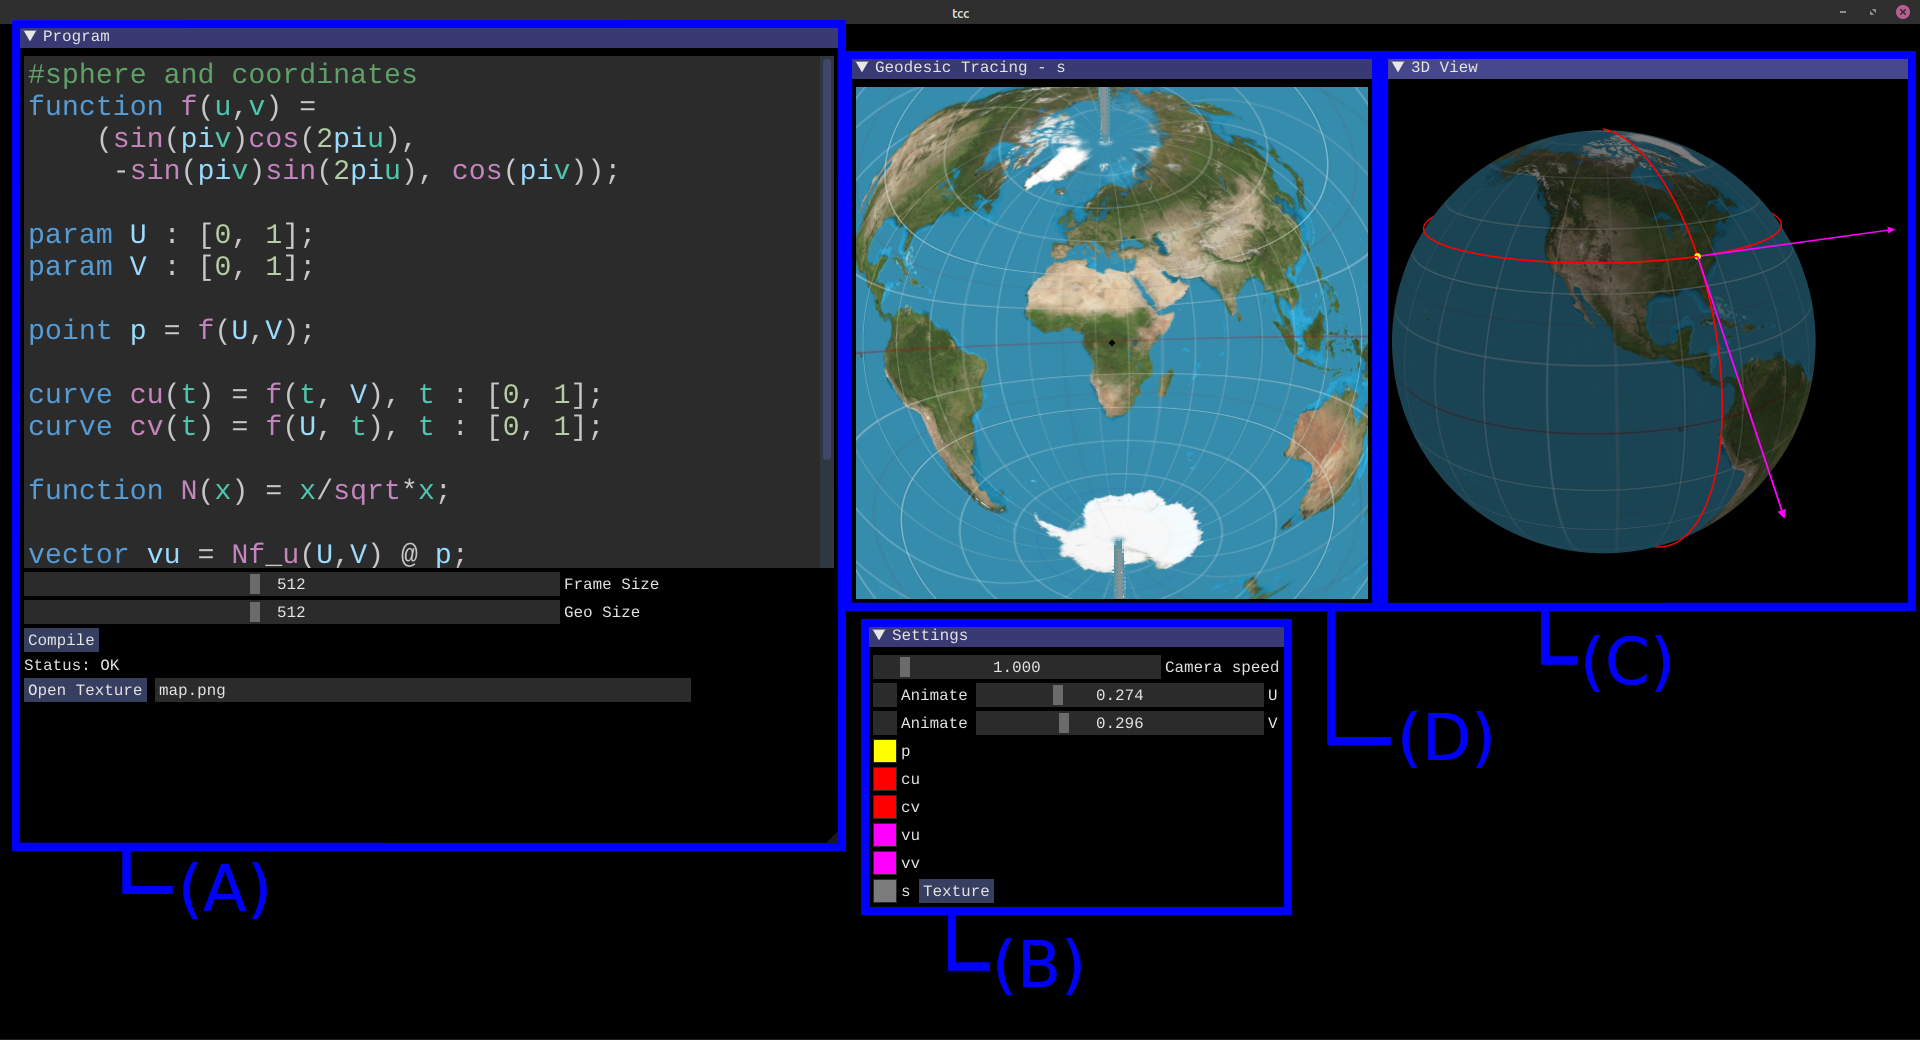
\includegraphics[width=\linewidth, frame]{comp.png}
    \caption{Componentes da interface gráfica}
    \label{img:comp}
\end{figure}

A Janela (A) da Figura \ref{img:comp} ilustra a janela \texttt{"Program"}, que contém uma
caixa de texto multilinha, onde o usuário deve escrever o programa.
O botão \texttt{"Compile"} compila o texto escrito.
A resposta do compilador será \texttt{"Status: OK"} para um programa compilado 
corretamente, ou \texttt{"Status: ..."} com uma mensagem de erro, indicando a
linha e a coluna correspondentes.
Dois controles deslizantes definem o tamanho, em \textit{pixels}, da janela
de visualização 3D(\texttt{"Frame size"}) e do \textit{Geodesic Tracing}(\texttt{"Geo Size"}).
O botão \texttt{"Open Texture"} serve para carregar uma imagem local,
com o nome informado à caixa de texto justaposta.
Quando o programa é compilado corretamente, duas janelas extras são exibidas.

A Janela (B) da Figura \ref{img:comp} ilustra a janela \texttt{"Settings"},
que controla algumas propriedades dos objetos.
Para os parâmetros, um controle deslizante é criado, com a opção \texttt{"Animate"}.
Quando ativado, o parâmetro é controlado pelo tempo,
crescendo uma unidade por segundo.
Quando o limite superior do parâmetro é atingido,
o valor volta para o limite inferior.

Para cada objeto desenhável é possível escolher uma cor.

Para uma superfície, os componentes RGB da textura
são multiplicadas pelos componentes RGB da cor escolhida.
A cor branca deixa a textura inalterada,
e preto deixa a textura completamente preta.
Além disso, é possível escolher uma textura previamente carregada para
uma superfície. A textura padrão é a textura local de nome \texttt{"default.png"}.

A velocidade da câmera é controlada por \texttt{"Camera speed"}.

A Janela (C) da Figura \ref{img:comp} ilustra a janela \texttt{"3D View"},
que exibe os objetos desenháveis no espaço 3d a partir de uma câmera.
A câmera pode ser controlada da seguinte forma:

\begin{table}[ht]
\caption{Controles da câmera 3D}
\label{camctrl}
\begin{centering}
\begin{tabularx}{\textwidth}{||c|X||}
    \hline
    \texttt{W} & move a câmera para frente \\
    \hline
    \texttt{S} & move a câmera para trás \\
    \hline
    \texttt{A} & move a câmera para a esquerda \\
    \hline
    \texttt{D} & move a câmera para a direita \\
    \hline
    \texttt{Q} & move a câmera para cima (absoluto) \\
    \hline
    \texttt{E} & move a câmera para baixo (absoluto) \\
    \hline
    \texttt{Clicar e mover} & gira a câmera conforme o movimento do mouse \\
    \hline
\end{tabularx}
\end{centering}
\end{table}

A renderização dos objetos utiliza um anti-serrilhado, melhorando sua estética.
Além disso, o desenho das linhas considera uma grossura que leva
em consideração a perspectiva, assim como os pontos e vetores.

Para uma superfície \texttt{\textit{x}}, a janela \texttt{"Geodesic Tracing - \textit{x}"} é exibida.
A janela exibe a visualização do \textit{Geodesic Tracing},
e está ilustrada na Janela (D) da Figura \ref{img:comp}.

A câmera pode ser controlada da seguinte forma:

\begin{table}[ht]
\caption{Controles do \textit{Geodesic Tracing}}
\label{gtctrl}
\begin{centering}
\begin{tabularx}{\textwidth}{||c|X||}
    \hline
    \texttt{W} & move a câmera para frente \\ 
    \hline
    \texttt{S} & move a câmera para trás \\
    \hline
    \texttt{A} & move a câmera para a esquerda \\
    \hline
    \texttt{D} & move a câmera para a direita \\
    \hline
    \texttt{Q} & gira a câmera no sentido anti-horário \\
    \hline
    \texttt{E} & gira a câmera no sentido horário \\
    \hline
    \texttt{Z} & zoom in \\
    \hline
    \texttt{X} & zoom out \\
    \hline
    \texttt{Clicar e mover} & move a câmera conforme o movimento do mouse \\
    \hline
\end{tabularx}
\end{centering}
\end{table}

Dependendo da expansão ou contração da imagem gerada no \textit{Geodesic Tracing},
o tamanho dos \textit{pixels} pode ficar grandes ou pequenos demais. O primeiro caso
deixa os \textit{pixels} individuais evidentes, e o segundo gera ruído, pois \textit{pixels} distantes
de cores muito diferentes `competem' para serem exibidos.
A exibição da textura é feita com filtro de magnificação linear, fazendo as transições
de \textit{pixels} grandes mais suave, resolvendo o primeiro problema.
O segundo problema foi resolvido com a técnica de \textit{mipmapping} linear.
Nessa técnica, a textura é copiada em resoluções progressivamente menores.
Por exemplo, um tabuleiro de xadrez possui casas brancas e pretas, e sua menor resolução
é apenas um \textit{pixel} cinza. Desse modo, quando a textura está muito contraída, 
uma versão de resolução menor é usada, resolvendo o ruído.
Essas técnicas podem ser facilmente obtidas configurando o \textit{OpenGL},
como pode ser observado em \cite{LearnOpenGL}.
